\documentclass[a4paper,zihao=5,UTF8]{ctexart}
\usepackage[top=2.3cm,bottom=2cm,left=1.7cm,right=1.7cm]{geometry} 
\usepackage{amsmath, amssymb}
\usepackage{color}
\usepackage{hyperref} 
\usepackage{pythonhighlight}
\usepackage{listings}
\usepackage{mathrsfs} 
\usepackage{booktabs}
\usepackage{amsthm}
\usepackage{longtable} 
\usepackage{graphicx}
\usepackage{subfigure}
\usepackage{caption}
\usepackage{fontspec}
\usepackage{titlesec}
\usepackage{fancyhdr}
\usepackage{latexsym}
\usepackage{subfigure}
\usepackage{braket}
\usepackage{cite}
\usepackage[version=4]{mhchem}

\CTEXsetup[format={\Large\bfseries}]{section}
\def\d{\mathrm{d}}
\def\e{\mathrm{e}}
\def\i{\mathrm{i}}
\def\dps{\displaystyle}
\newcommand{\mr}[1]{\mathrm{#1}}
\newcommand{\mb}[1]{\mathbf{#1}}
\newcommand{\dv}[2]{\frac{\d{#1}}{\d{#2}}}
\newcommand{\pdv}[2]{\frac{\partial{#1}}{\partial{#2}}}
\def\degree{$^{\circ}$}
\def\celsius{^{\circ}\mr{C}}
\title{\textbf{实验五 用对-叔丁基杯[8]芳烃分离\ce{C_{60}}
\cite{inorganic_chemistry_1}}}
\author{王崇斌\;1800011716}
\makeatletter
\makeatother
\begin{document}
	\pagestyle{fancy}
	\pagestyle{fancy}
    \lhead{无机化学实验}
	\chead{}
	\rhead{\today}
	\maketitle
    \thispagestyle{fancy}
    \section{实验目的}
    \begin{enumerate}
        \item 了解超分子化学在化学分离中的应用
        \item 了解杯芳烃的合成
        \item 了解杯芳烃分离\ce{C_{60}}与\ce{C_{70}}的原理与方法
    \end{enumerate}
	\section{实验原理}
    \subsection{杯芳烃的合成}
    杯芳烃因其酒杯状的结构而得名,这类分子具有大小可调节的\textbf{空腔},能够有选择性的
    和尺寸不同的分子或离子形成主客体复合物。随着烃基的不同或者通过衍生化,
    可以获得多种类型的杯芳烃,它们在极性或者非极性溶剂中有着不同的溶解性,
    可以满足各种特定的需求。对-叔丁基杯芳烃是杯芳烃中最具代表性、最常见的一种,
    根据苯环的数目分别命名为杯芳烃四、杯芳烃六、杯芳烃八(图\ref{calixarene})。
    \begin{figure}[htbp]
        \centering
        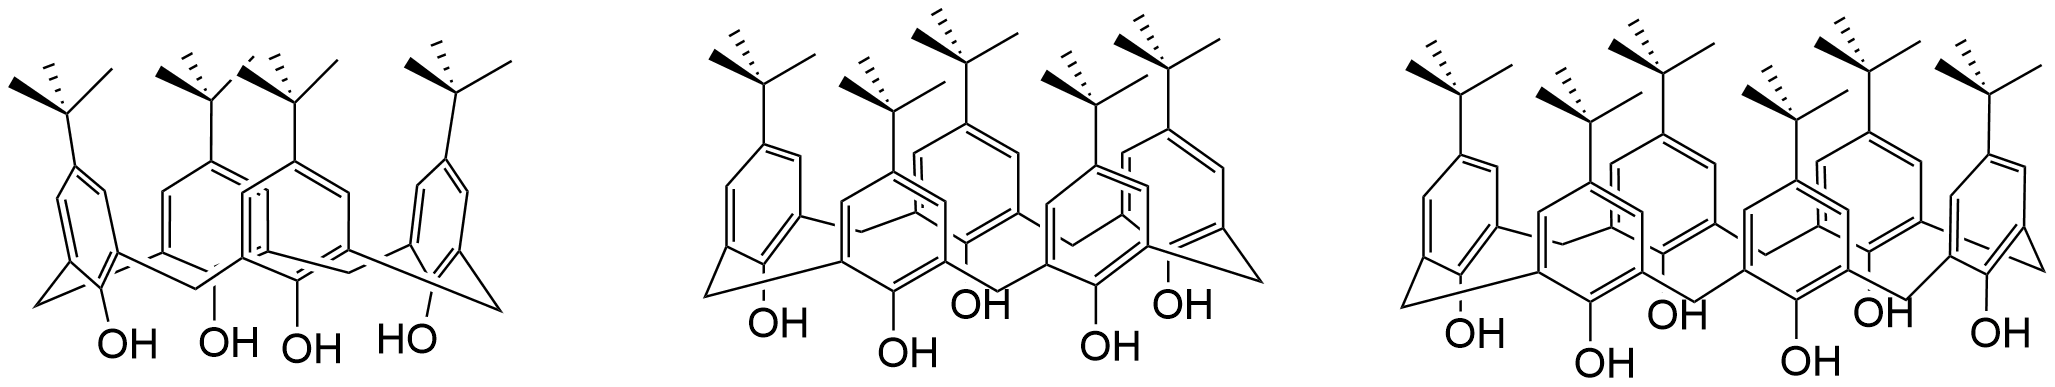
\includegraphics[scale=0.3]{calixarene.png}
        \caption{杯芳烃四、杯芳烃六、杯芳烃八结构示意图}
        \label{calixarene}
    \end{figure}
    \par 
    对-叔丁基杯芳烃是由对-叔丁基苯酚和甲醛在一定条件下缩合而成。
    \subsection{杯芳烃选择性分离\ce{C_{60}}与\ce{C_{70}}的原理}
    杯芳烃可以选择性地和富勒烯形成配合物,如对-叔丁基杯[8]芳烃与\ce{C_{60}}形成1:1
    配合物,对-叔丁基杯[6]芳烃与\ce{C_{70}}形成1:2配合物。这是因为对-叔丁基杯[8]芳烃
    的杯形空腔大小与\ce{C_{60}}的直径相匹配,而且苯环和富勒烯之间也有着比较强的相互作用。
    杯[8]芳烃-\ce{C_{60}}的配合物,不溶于甲苯,可以从甲苯中析出;但是配合物可以在氯仿中
    解离,因为杯芳烃易溶于氯仿,此时\ce{C_{60}}变为沉淀析出。利用这个原理,可以利用
    杯芳烃从富勒烯混合物中分离\ce{C_{60}}。

    \section{实验内容}
    实验时间:2021年4月23日
    \par
    实验地点:北京大学化学与分子工程学院D区三楼第八实验室2号实验台
    \subsection{从富勒烯混合物中分离和纯化\ce{C_{60}}}
    称取富勒烯混合物100mg(102mg)置于锥形瓶中,加入80ml(81ml)甲苯超声溶解。溶解一定时间后,
    将混合物过滤到圆底烧瓶中,此时溶液呈现出深紫红色。
    在滤液中加入216mg对-叔丁基杯[8]芳烃,超声20-30min充分溶解,随后离心弃去母液,母液为
    红棕色,沉淀颜色很深(不好分辨具体是什么颜色)。
    \par 
    用50ml甲苯转移沉淀至圆底烧瓶中,加热回流至悬浮物充分溶解(但是避免长时间回流),溶解后
    在溶液中补加50mg杯芳烃。将回流后的溶液超声20-30min,出现大量的沉淀,离心分离,弃去
    上层清液,将甲苯挥干,得到黄绿色固体。用10ml甲苯洗涤沉淀2次,直到上层清液几乎无色。
    最后一次洗涤分离甲苯之后加入石油醚(方便甲苯的挥发),等待沉淀干燥,可以观察到
    离心试管中固体显示出金黄色。在其中加入<20ml的氯仿,将固体重新悬浮,置于水浴(~60$\celsius$)
    中加热溶解,溶液颜色明显变浅为淡紫色,沉淀为黑色颗粒状,离心分离得到\ce{C_{60}}。
    \subsection{测定产品\ce{C_{60}}的纯度与含量}
    用20mL甲苯将产物转入50mL容量瓶,加甲苯定容至刻线,摇匀备用。用滴管取0.5mL\ce{C_{60}}
    溶液,在5mL比色管中定容,摇匀。将比色管与标准色阶对比,确定产品纯度,经过比较,
    实验者所的产品的纯度大于99.9\%,对比结果如图\ref{compare}所示。
    \begin{figure}[htbp]
        \centering
        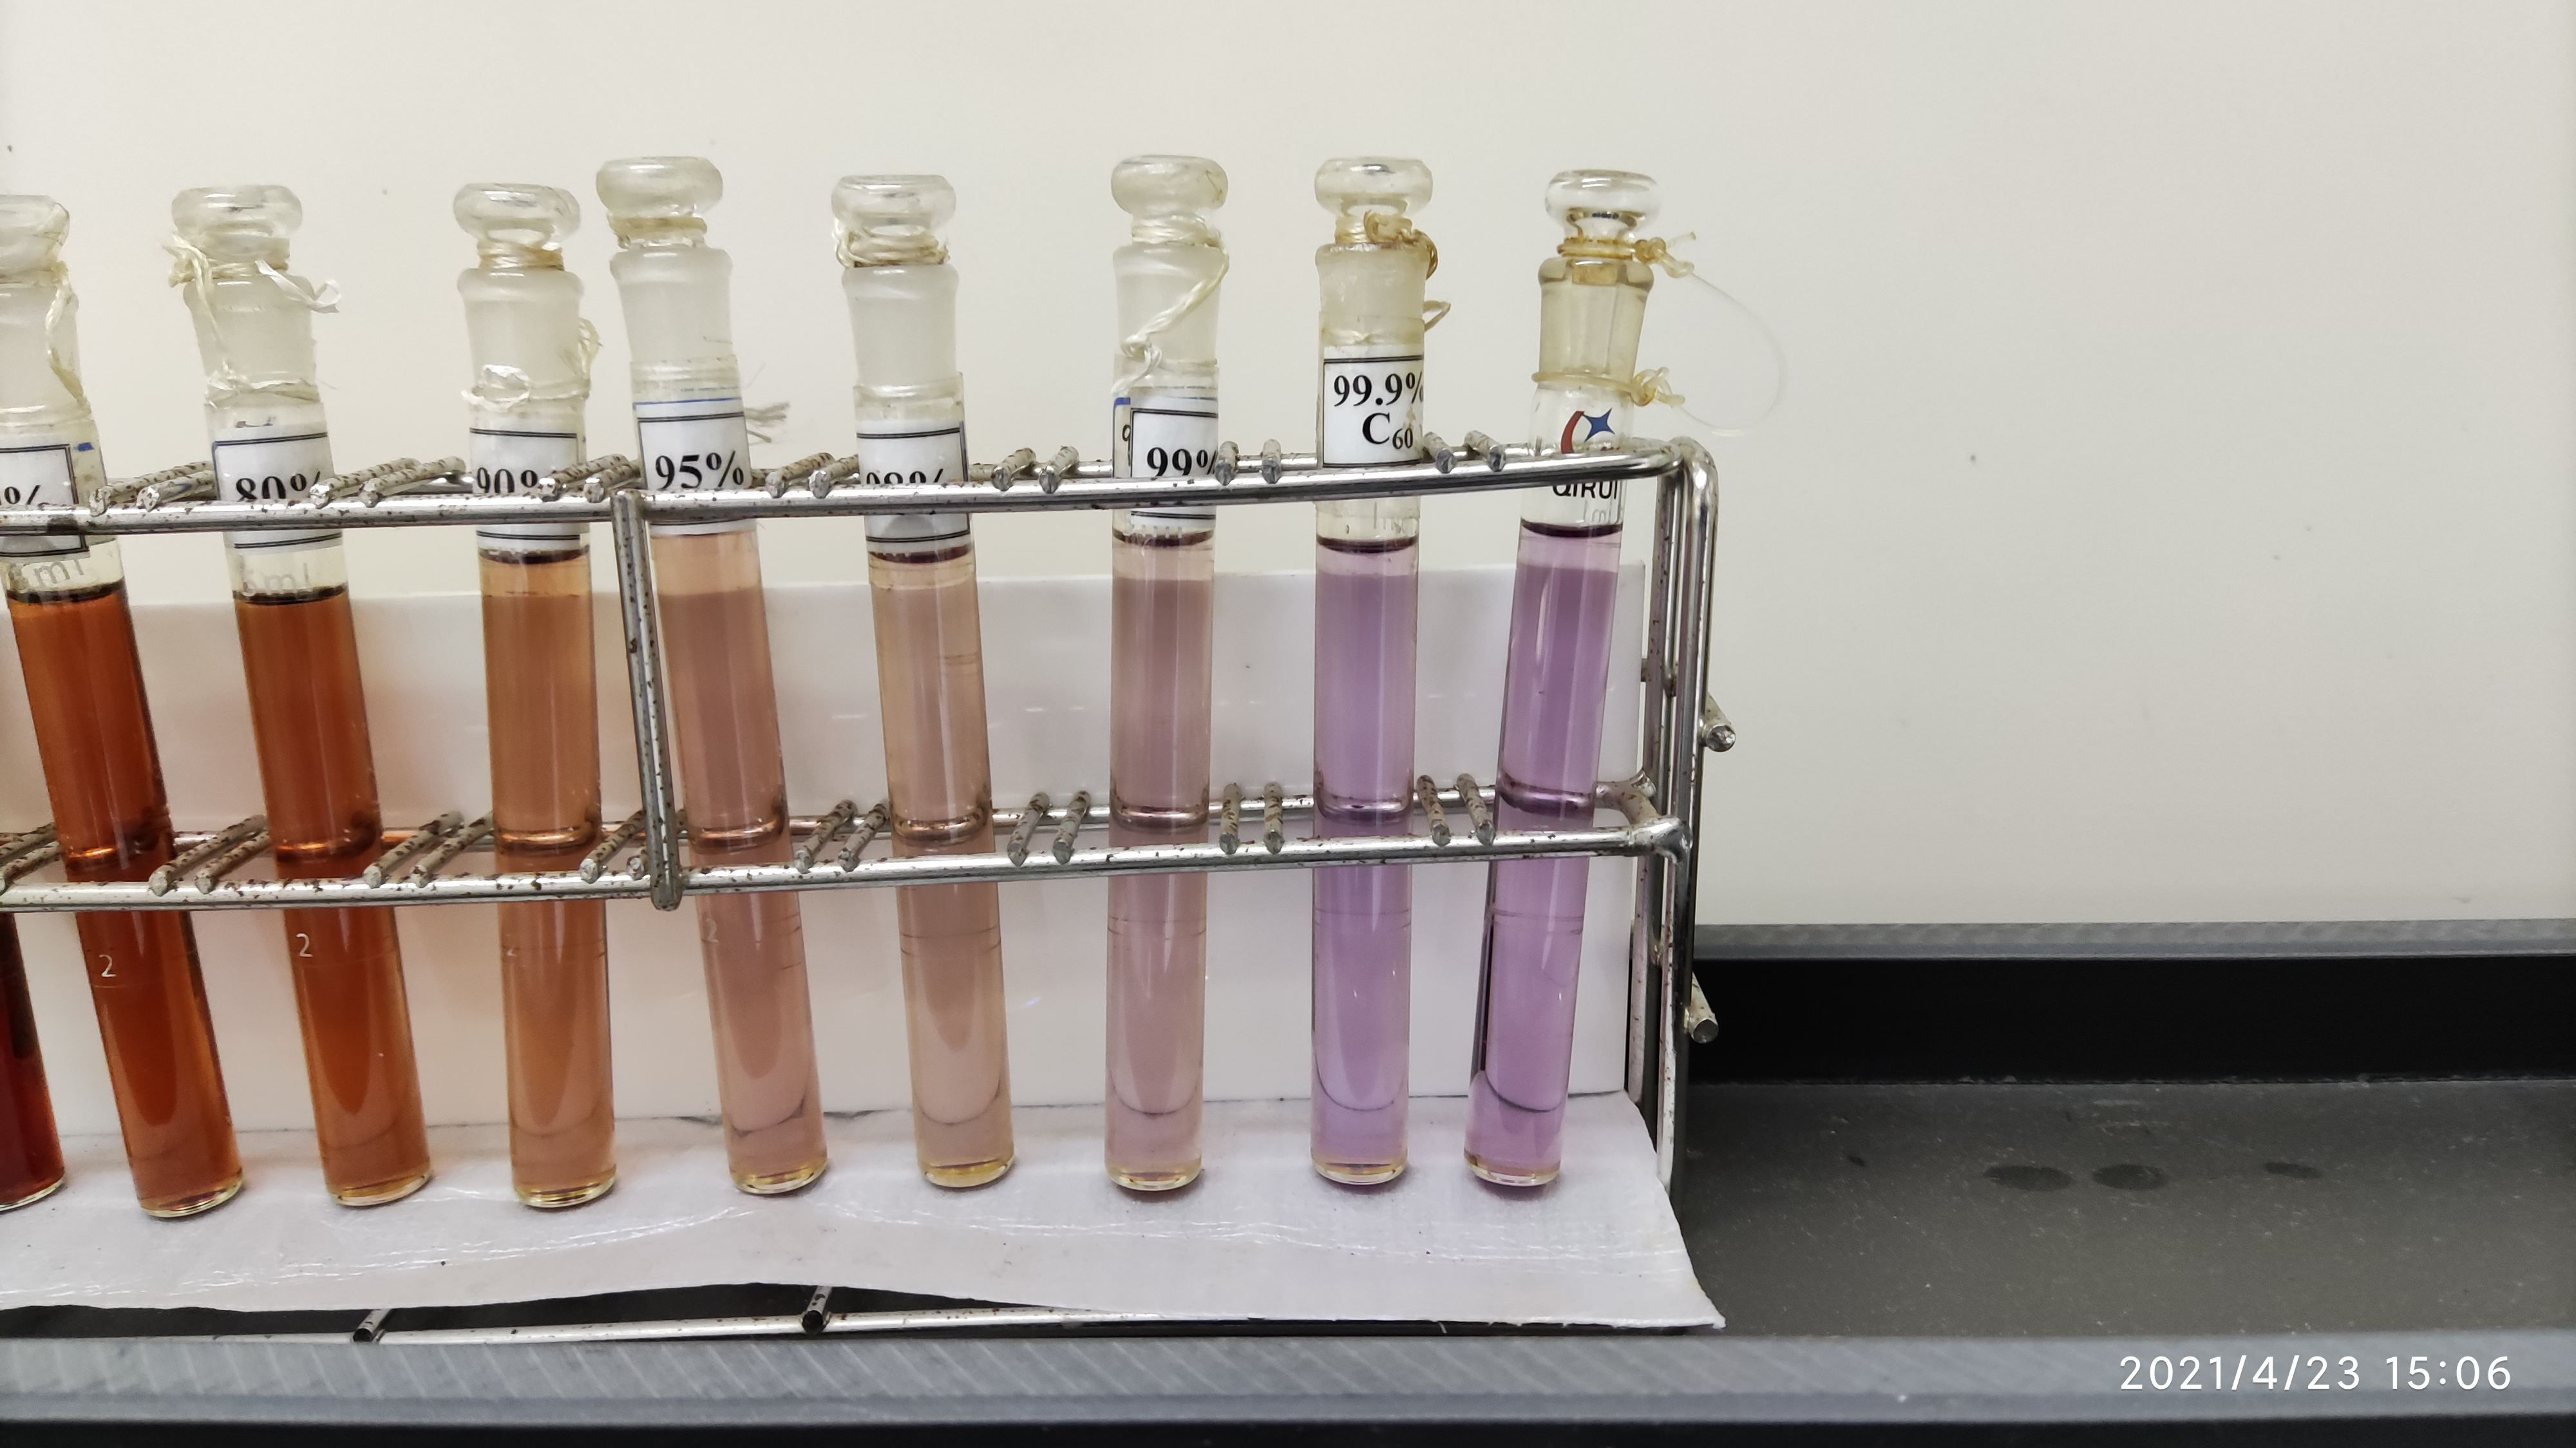
\includegraphics[scale=0.1]{compare.jpg}
        \caption{目视比色法判断\ce{C_{60}}纯度}
        \label{compare}
    \end{figure}
    用微量进样器取50μL\ce{C_{60}}溶液,在10mL容量瓶中用甲苯定容,摇匀。
    用紫外可见分光光度计中测定335nm处的吸光度,由工作曲线确定浓度,并计算分离的收率。
    分光光度法测得溶液(最后一步用微量进样器配置的溶液)浓度为0.0052g/L,对应原混合物中
    有52mg\ce{C_{60}},回收率为:51\%。
    \section{结果与讨论}
    \paragraph{(1)}\textbf{计算\ce{C_{60}}甲苯溶液中的\ce{C_{60}}含量和收率}
    \par 在实验步骤中已经讨论了。从实验室的整体情况来看,同学们分离得到的\ce{C_{60}}
    纯度都非常高,且回收率大多都在50\%之上,说明用杯芳烃分离富勒烯混合物确实是一种
    高效的方法。
    \paragraph{(2)}\textbf{讨论加热回流和超声在对-叔丁基杯[8]芳烃分离\ce{C_{60}}
    与\ce{C_{70}}中的作用}
    \par 回流这一步操作在首次得到杯芳烃-\ce{C_{60}}复合物之后进行,这步操作是为了
    让复合物分解,从而在下一步超声中重新生成复合物。因为首次从富勒烯混合物中生成的
    复合物中必然包藏了比较多的\ce{C_{60}}以外的富勒烯,通过这样一部“重新沉淀”的过程,
    可以减小复合物中其他富勒烯的包藏,提高产物的纯度(但是相应的,由于富勒烯和复合物
    在甲苯中的溶解,这样一定会降低收率)。超声在两次生成复合物的过程中都有使用,
    其目的是高效、均匀地混合反应体系,大大减小复合物生成所需要的时间。
    \paragraph{(3)}\textbf{根据附图2讨论对-叔丁基杯[8]芳烃分离\ce{C_{60}}和
    \ce{C_{70}}的效率,能否做到\ce{C_{60}}和
    \ce{C_{70}}的完全分离(收率和纯度都达到99\%)?如何做到?}
    \par 显然不能做到完全分离,因为在首次从富勒烯混合物的甲苯溶液中沉淀复合物之后的母液中
    就含有13.70\%的\ce{C_{60}}(相对含量),如果假设在分离中不损失\ce{C_{70}},可以
    计算出在母液中的\ce{C_{60}}占所有\ce{C_{60}}的比例为3.3\%,因此无论如何都不能完全分离。
    通过本次实验验证,分离的到的富勒烯已经满足了纯度的要求。

    \section{思考题}
    \paragraph{(1)}\textbf{杯芳烃分离富勒烯是否达到了热平衡?请设计一个实验证明
    方案}
    \par 
    设置其他条件相同、超声时间不同的多组反应,观察第一次离心后母液中的富勒烯比例。
    如果随着反应时间延长,比例趋向一个定值,则说明达到热平衡。
    \paragraph{(2)}\textbf{杯[8]芳烃和\ce{C_{60}}甲苯溶液在超声的作用下生成配合物沉淀
    ,解释超声在其中所起的作用,并于其他促进反应的方法(如搅拌、加热搅拌)做优劣比较}
    \par 
    超声波长远大于分子的尺度,所以超声波并不直接与反应物相互作用(这里指区别于光照,
    超声并不参与直接的化学过程)。普遍认为,超声能促进反应是因为“空化作用”:
    超声波在液体中可能以驻波形式存在,在溶液中会形成局部的高密度和低密度交替的区域,
    液体内局部出现拉应力而形成负压,压强的降低使原来溶于液体的气体过饱和,
    而从液体逸出,成为小气泡(超声波加湿器),在溶液分子被震荡产生气泡的过程中,
    反应物得到了充分的混合,由于超声波波长短,相较于机械搅拌,这是更小尺度上的充分混合,
    因此可以明显加速很多受扩散控制的反应的速度。
    \par 
    与加热相比,超声可以不用加热,有可能更加适用于对热敏感的反应体系,而且从能耗的角度
    来考虑,超声有可能更加省电,如果从仪器价格的角度来考虑,超声可能比传统的加热手段更加
    经济。与搅拌相比,机械搅拌可能促进反应的效率略低,但是对于较大的反应剂量(比如工业生产)
    ,机械搅拌还是更加有优势。
    \paragraph{(3)}\textbf{\ce{C_{70}}在杯[8]芳烃的配合物中是吸附状态还是配合状态?
    如何证明}
    \par 
    个人认为是吸附状态,如果是配合状态,那么应该与\ce{C_{60}}复合物一样,应该能从甲苯中
    沉淀出来,但是事实上并没有。可以对加入了杯芳烃的富勒烯甲苯溶液做紫外吸收光谱的研究,
    配合状态的\ce{C_{70}}光谱应有明显变化。
    \paragraph{(4)}\textbf{影响\ce{C_{60}}纯度的主要因素是什么?用对-叔丁基杯[8]芳烃
    提纯\ce{C_{60}}有没有极限?要使\ce{C_{60}}的纯度达到99\%之上,重结晶是否必要(最好用
    实验说明)?}
    \par 
    影响\ce{C_{60}}纯度的主要因素是各步离心分离和洗涤时有没有将沉淀和母液尽可能分离
    (主要是用甲苯洗涤沉淀那一步是否洗涤地充分),还有让复合物溶解后重新沉淀的步骤
    也相当重要。提纯是有极限的,复合物总会吸附少量\ce{C_{70}}和富勒烯氧化物。为了
    提高纯度,重结晶复合物显然是不会提高纯度的,重结晶最后得到的富勒烯不太现实,因为量太小,
    会产生极大的损失。要提高纯度还是应当考虑将最后一步得到的富勒烯用甲苯溶解后通过色谱分离。
    \paragraph{(4)}\textbf{请解释各阶段所生成的沉淀的颜色变化的原因}
    \par 
    最开始配制的富勒烯混合物溶液,颜色为很深的棕红色,这是\ce{C_{70}}和\ce{C_{60}}溶解
    在甲苯中的混合色,这个可以通过观察标准色阶的比色管看出,混合有两种富勒烯的甲苯溶液
    会明显偏离紫红色而呈现出红棕色,在未加入杯芳烃之前,富勒烯并没有完全溶解,可以看到
    有少量深色沉淀在锥形瓶底部。
    \par 
    在第一次加入杯芳烃而后离心弃去母液的过程中,可以观察到离心管上清液为红棕色
    (溶液颜色明显比上一步要浅很多),沉淀为深红棕色(接近黑色),具体情况参考图
    \ref{color}。
    \begin{figure}[htbp]
        \centering
        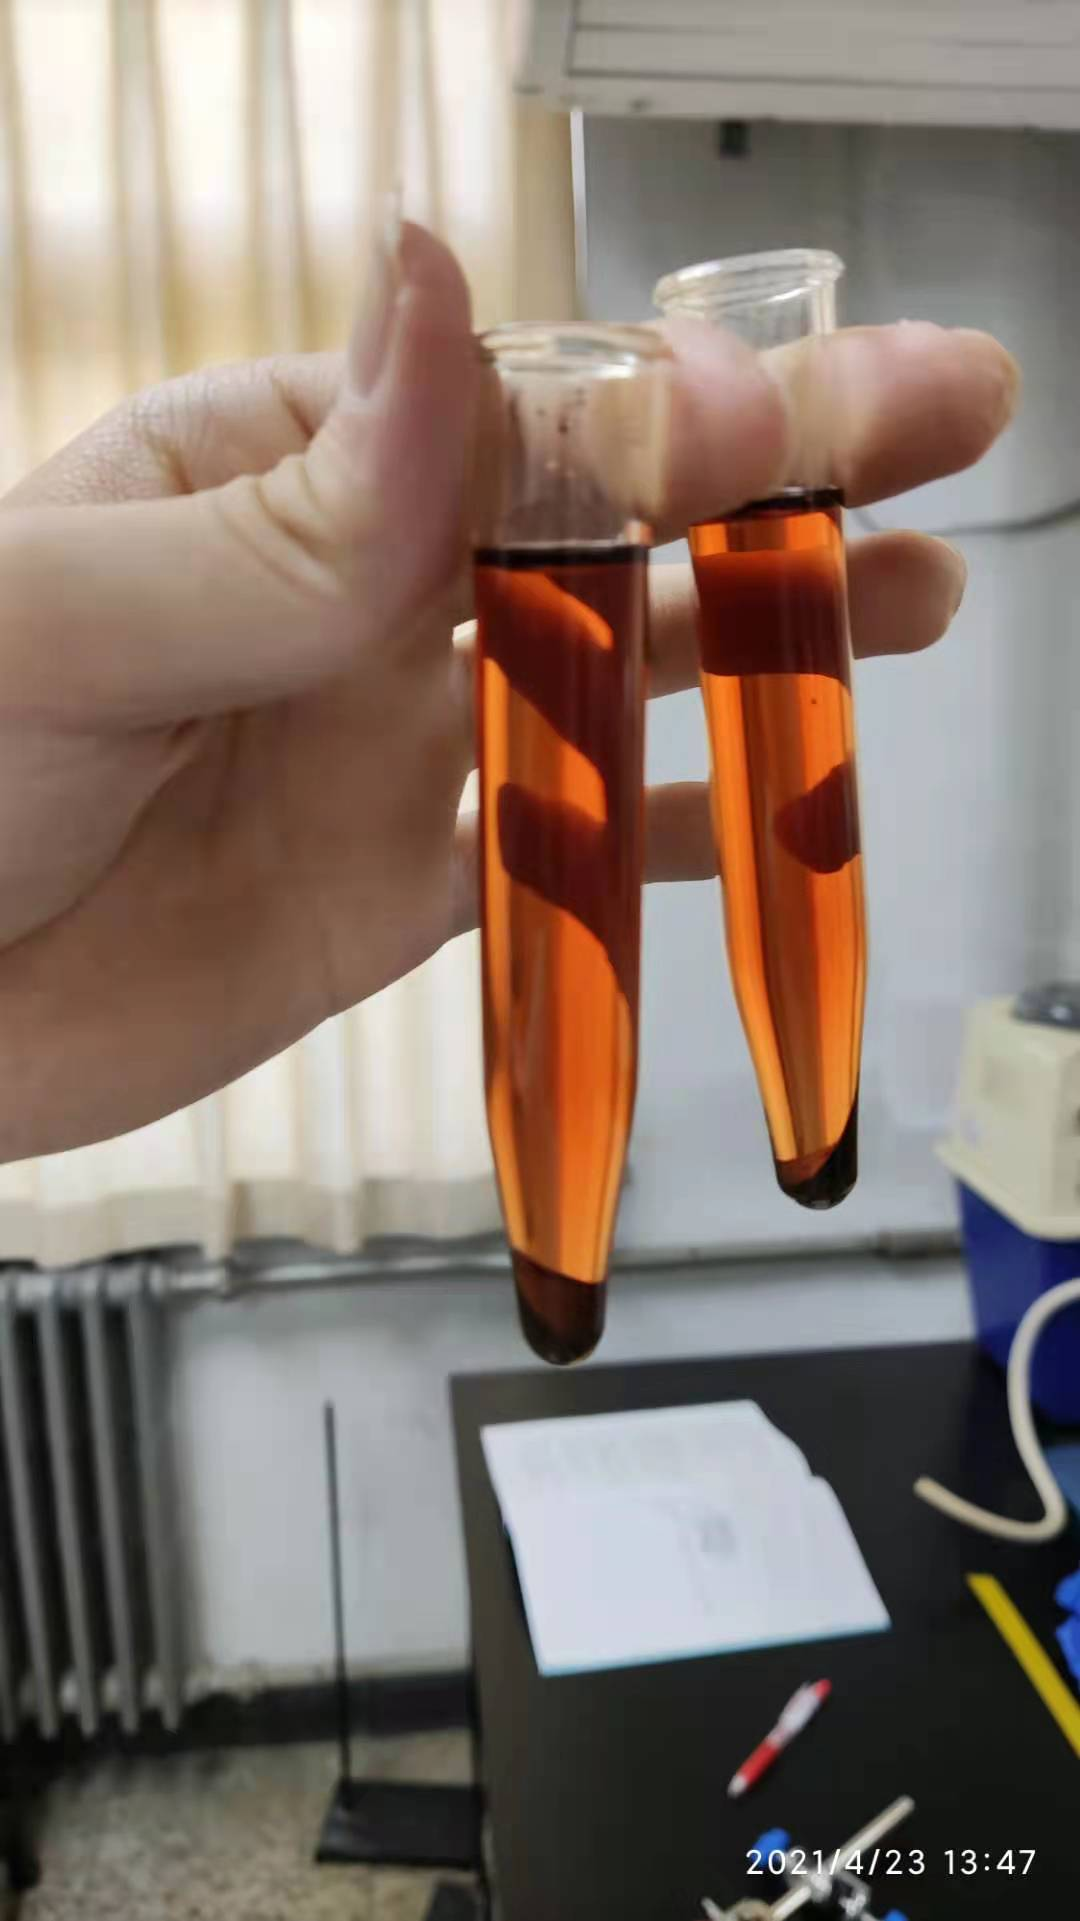
\includegraphics[scale=0.15]{color.jpg}
        \caption{加入杯芳烃后体系的颜色}
        \label{color}
    \end{figure}
    \par 
    在将上述沉淀重新溶解,补加杯芳烃,将体系超声后重新产生的沉淀,经过离心分离后呈现出
    黄绿色。将上述黄绿色沉淀用甲苯充分洗涤后,挥干甲苯得到的产物为金黄色,具体情况参考图
    \ref{color2}。
    \begin{figure}
        \centering
        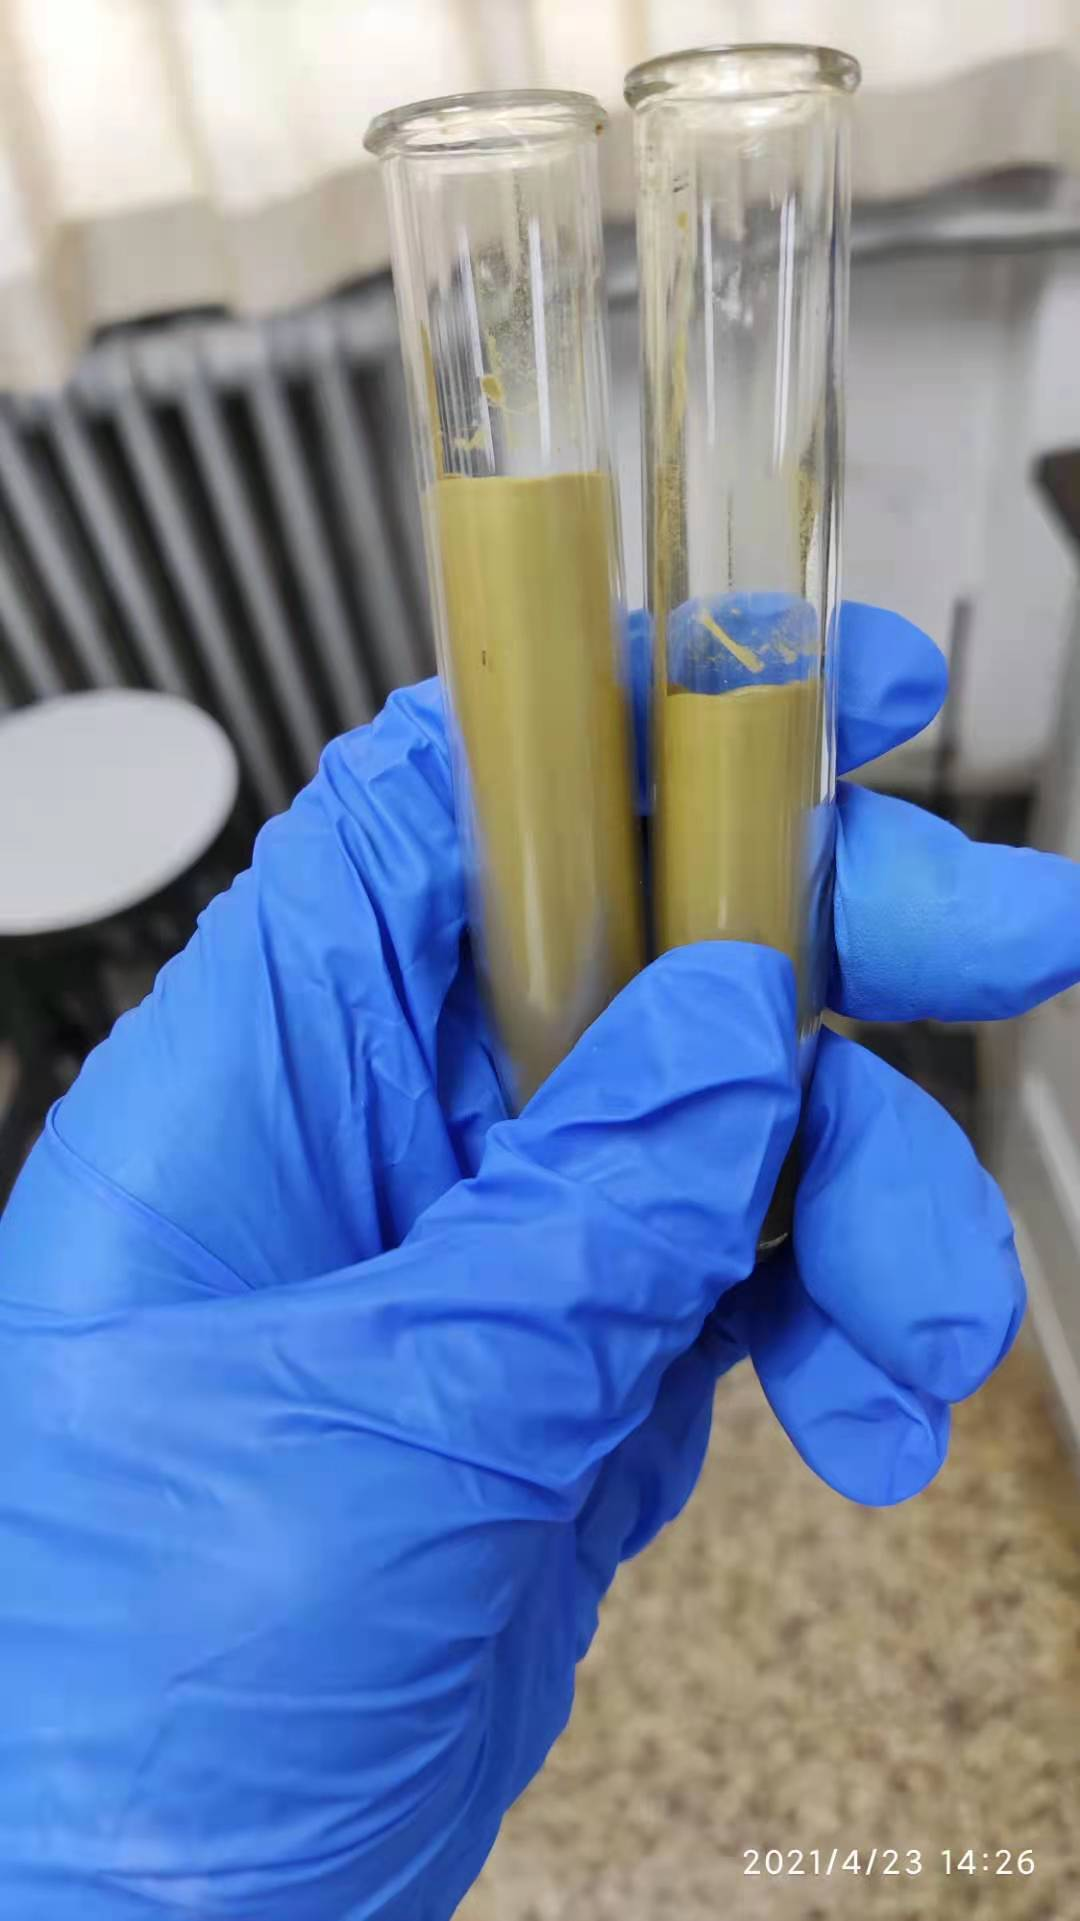
\includegraphics[scale=0.15]{color2.jpg}
        \caption{杯芳烃-\ce{C_{60}}复合物的颜色}
        \label{color2}
    \end{figure}
    \par 
    最后一步向上述复合物中加入氯仿并加热,复合物分解,杯芳烃溶于氯仿而\ce{C_{60}}变为沉淀、
    深紫黑色(像高锰酸钾),溶液由于有少量\ce{C_{60}}溶解也呈现出淡紫色。
    \paragraph{(5)}\textbf{本实验甲苯溶液需回收使用,但是甲苯中混入少量氯仿就无法完成
    分离过程,为什么?}
    \par 
    在实验的最后一步,通过使用氯仿破坏配合物的方式使\ce{C_{60}}游离出来(当然也利用了
    \ce{C_{60}}在氯仿中几乎不溶解的事实),这说明杯芳烃在氯仿中有着极大的溶解度,
    极大地拉动了复合物的配位-解离平衡向解离方向移动。如果在甲苯溶液中混有氯仿,
    这不仅会使得富勒烯在其中难以溶解,同时会极大地抑制复合物的生成,降低分离效率,因此
    甲苯中混有少量氯仿就会无法完成分离过程。


    \bibliographystyle{plain}
	\bibliography{ref}
\end{document}